% Provenance (never printed): see sources/outline_sources.md (Year 3:
% ocean dynamics: the Ekman layer derived, the Sverdrup balance, western
% intensification, the abyssal circulation, ocean tides).
% Brief: sources/book5/BRIEFS.md, ch. 21. Curves from
% figdata/bachelor-3/wind_driven_gyre.py and tides.py. Exercise and problem
% values in the Book 5 scratch calculator calc/ch21.py. The basins, winds
% and stations of the exercises and the problem are invented.
\chapter{Dynamique océanique}\label{ch:b3:ocean-dynamics}

Par le détroit de Floride, le Gulf Stream transporte environ
\qty{32}{\sverdrup} d'eau vers le nord, et son débit croît en longeant la côte
vers le nord, jusqu'à environ \qty{150}{\sverdrup} vers \ang{40}~N. De l'autre côté du même océan, au large du Portugal et du nord
de l'Afrique, rien de comparable ne s'écoule vers le sud~: l'eau que le Gulf Stream transporte
vers le nord revient vers l'équateur sous la forme d'une dérive lente et large, à travers des milliers
de kilomètres de mer ouverte. Chaque bassin océanique de l'hémisphère Nord présente
la même forme dissymétrique, son courant rapide étant situé du côté ouest. La
dissymétrie découle du vent, du frottement de la mer et
d'un fait concernant la Terre~: le paramètre de Coriolis croît vers le pôle.
% ledger: rapid:transports (31.7 Sv, rounded), stewart:north-atlantic

\begin{recall}
La force de marée de la Lune et du Soleil, ainsi que les marées de vive-eau et de morte-eau, figurent dans les
volumes de physique. La tension du vent, la couche d'Ekman, le transport d'Ekman et
la spirale d'Ekman, la remontée et la plongée d'eau, les gyres, les courants de
bord ouest, le sverdrup ($\qty{1}{\sverdrup} =
\qty{e6}{m^3/s}$), la circulation méridienne de retournement et la
formation des eaux profondes figurent dans le volume de première année, dans son chapitre sur
la circulation océanique~; la tension du vent s'y écrit $\vec T$, ici
$\vec\tau$. Le paramètre de Coriolis, le plan $\beta$, le rayon de Rossby
et l'équilibre géostrophique figurent au chapitre~\ref{ch:b3:gfd-foundations}~;
la vorticité et la \omterm{def:b3:atmospheric-dynamics:pv}{vorticité potentielle} sont au chapitre~\ref{ch:b3:atmospheric-dynamics}.
\end{recall}

\section{La couche d'Ekman démontrée}\label{sec:b3:ocean-dynamics:ekman}

Dans le volume de première année, le transport d'Ekman avait été obtenu à partir d'un bilan des forces
sur toute la couche, et la spirale des vitesses à l'intérieur de celle-ci était énoncée. Avec
un frottement turbulent de viscosité verticale constante $A_z$, la spirale découle
des équations en quelques lignes. On écrit la vitesse horizontale sous la forme
d'un nombre complexe, $W = u + \mathrm iv$, et la tension du vent comme $\tau =
\tau_x + \mathrm i\tau_y$~; la multiplication par $-\mathrm i$ fait tourner un vecteur
de \ang{90} dans le sens horaire, c'est-à-dire vers sa droite vue d'en haut.

\begin{theorem}[Profil de vitesse d'une couche de surface stationnaire entraînée par le vent]\label{thm:b3:ocean-dynamics:ekman}
Dans un océan stationnaire, horizontalement uniforme, de grande profondeur et de masse volumique constante
$\rho$, avec une viscosité turbulente verticale constante $A_z$ et le paramètre de Coriolis
$f > 0$, le courant entraîné par une tension du vent $\tau$ s'écrit
\[
W(z) = W_0\,\mathrm e^{(1+\mathrm i)z/\delta},\qquad
W_0 = \frac{\tau}{\rho\sqrt{fA_z}}\,\mathrm e^{-\mathrm i\pi/4},\qquad
\delta = \sqrt{\frac{2A_z}{f}} ,
\]
pour $z \le 0$. Le courant de surface est tourné de \ang{45} vers la droite de la
tension~; avec la profondeur, il tourne davantage vers la droite et décroît comme $\mathrm
e^{z/\delta}$~; le transport total $\int_{-\infty}^0 W\,\mathrm dz =
-\mathrm i\tau/(\rho f)$ est perpendiculaire à la tension, vers sa droite.
\end{theorem}

\begin{proof}
Loin des côtes, il n'existe aucun gradient horizontal de pression dans la couche,
et la force de Coriolis équilibre le frottement~: $-fv = A_z u''$ et $fu =
A_z v''$, les primes désignant des dérivées en $z$. En multipliant la seconde par
$\mathrm i$ et en additionnant, on obtient $A_zW'' = \mathrm ifW$. Ses solutions sont
$\mathrm e^{\pm(1+\mathrm i)z/\delta}$, car $(1+\mathrm i)^2/\delta^2 =
2\mathrm i/\delta^2 = \mathrm if/A_z$~; seul le signe plus reste borné lorsque
$z \to -\infty$. À la surface, la tension est transmise par le frottement,
$\rho A_zW'(0) = \tau$, d'où $W_0 = \tau\delta/(\rho A_z(1+\mathrm i))$.
Comme $\delta/(\sqrt2 A_z) = 1/\sqrt{fA_z}$ et $1/(1+\mathrm i) = \mathrm
e^{-\mathrm i\pi/4}/\sqrt2$, on retrouve le $W_0$ énoncé. Le facteur
$\mathrm e^{\mathrm iz/\delta}$ tourne dans le sens horaire lorsque $z$ diminue. Enfin
$\int_{-\infty}^0 W\,\mathrm dz = W_0\delta/(1+\mathrm i) =
\tau\delta^2/(\rho A_z(1+\mathrm i)^2) = \tau\delta^2/(2\mathrm i\rho A_z)
= -\mathrm i\tau/(\rho f)$.
\end{proof}

Le théorème retrouve les deux résultats du volume de première année~: le courant de surface d'Ekman
à \ang{45}, et le transport $\tau/(\rho f)$, perpendiculaire à
la tension et indépendant de $A_z$, qui n'est jamais bien connu. À la
profondeur $\pi\delta$, le courant circule à contre-sens du courant de surface, réduit
d'un facteur $\mathrm e^{-\pi}$, soit \qty{4}{\percent}.

\begin{definition}[Profondeur d'Ekman~; pompage d'Ekman]\label{def:b3:ocean-dynamics:ekman-pumping}
La \emph{profondeur d'Ekman}\index{profondeur d'Ekman} est $D_E = \pi\delta =
\pi\sqrt{2A_z/f}$, la profondeur à laquelle le courant de la spirale d'Ekman
circule à contre-sens du courant de surface~; elle mesure l'épaisseur de la
couche d'Ekman. Le \emph{pompage d'Ekman}\index{pompage d'Ekman} est la vitesse
verticale $w_E$ à la base de la couche d'Ekman, imposée par la convergence ou
la divergence du transport d'Ekman~: vers le bas là où les transports
convergent, vers le haut, parfois appelée succion d'Ekman, là où ils divergent.
\end{definition}

\begin{proposition}[Pompage d'Ekman]\label{prop:b3:ocean-dynamics:pumping}
La vitesse verticale étant nulle à la surface de la mer, le \omterm{def:b3:ocean-dynamics:ekman-pumping}{pompage d'Ekman} est
\[
w_E = \operatorname{curl}_z\frac{\vec\tau}{\rho f}
= \frac{1}{\rho f}\Big(\frac{\partial\tau_y}{\partial x} -
\frac{\partial\tau_x}{\partial y}\Big) + \frac{\beta\tau_x}{\rho f^2} ,
\]
comptée positivement vers le haut.
\end{proposition}

\begin{proof}
Le transport volumique de la couche vaut $(U_E, V_E) = (\tau_y,
-\tau_x)/(\rho f)$, c'est le théorème écrit en composantes. En intégrant
l'équation de continuité $\partial w/\partial z = -(\partial u/\partial x +
\partial v/\partial y)$ à travers la couche, $w(0) - w_E = -(\partial
U_E/\partial x + \partial V_E/\partial y)$, donc $w_E = \partial_x(\tau_y/\rho
f) - \partial_y(\tau_x/\rho f)$. En développant avec $\mathrm df/\mathrm dy =
\beta$, on obtient la seconde forme.
\end{proof}

Un vent tournant de façon cyclonique au-dessus de la mer, dont le rotationnel est positif, aspire
de l'eau depuis le dessous de la couche~; un vent anticyclonique la refoule vers le bas. Au-dessus
des océans subtropicaux, les alizés soufflent d'est du côté équatorial, les
vents d'ouest soufflent depuis l'ouest du côté polaire. Leurs transports d'Ekman
vers le nord sous les alizés et vers le sud sous les vents d'ouest,
convergent entre eux~: l'eau de surface s'accumule et est refoulée vers le bas, comme
sur la figure ci-dessous. Le long d'une côte où le
vent souffle avec la côte à sa gauche (dans l'hémisphère Nord), le
transport s'éloigne du rivage, et la remontée côtière du volume de première année
est une aspiration d'Ekman concentrée contre un mur.

\begin{omfigure}
\centering
\begin{tikzpicture}[>=stealth, font=\small, x=1.1cm, y=1cm]
\fill[omThm!7] (-5,0) rectangle (5,-3.6);
\draw[thick] (-5,0) -- (5,0);
\draw[black!45, densely dashed] (-5,-0.9) -- (5,-0.9);
\node[font=\scriptsize, black!60, anchor=north east, inner sep=1pt] at (4.95,-0.95) {couche d'Ekman};
% winds: west is out of the page, east into the page
\foreach \x in {-4.2,-3.4,-2.6} {\draw (\x,0.55) circle (0.13); \fill (\x,0.55) circle (0.04);}
\foreach \x in {2.6,3.4,4.2} {\draw (\x,0.55) circle (0.13);
  \draw (\x-0.09,0.46) -- (\x+0.09,0.64); \draw (\x-0.09,0.64) -- (\x+0.09,0.46);}
\node[above] at (-3.4,0.75) {alizés, venant de l'est};
\node[above] at (3.4,0.75) {vents d'ouest, venant de l'ouest};
% Ekman transports converge
\draw[->, omDef, very thick] (-4.5,-0.45) -- (-1.2,-0.45);
\draw[->, omDef, very thick] (4.5,-0.45) -- (1.2,-0.45);
\node[omDef, font=\scriptsize, fill=omThm!7, inner sep=1pt] at (-2.85,-0.72) {transport d'Ekman};
% pumping
\foreach \x in {-0.6,0,0.6} \draw[->, omThm, thick] (\x,-0.55) -- (\x,-1.55);
\node[omThm, font=\scriptsize, anchor=west] at (0.75,-1.25) {$w_E < 0$};
% squashed column and Sverdrup flow
\draw[thick, black!70] (-0.62,-1.75) rectangle (0.62,-3.1);
\node[font=\scriptsize, black!70, align=center] at (0,-2.42) {colonne\\comprimée};
\draw[->, omMeth, very thick] (-0.75,-2.42) -- (-3.2,-2.42);
\node[omMeth, font=\scriptsize, align=center, above] at (-2.6,-2.40) {écoulement de Sverdrup,\\vers l'équateur};
\draw[black!45, densely dashed] (-5,-3.3) -- (5,-3.3);
\node[font=\scriptsize, black!60, anchor=south east, inner sep=1pt] at (4.95,-3.28) {base de l'écoulement entraîné par le vent};
\node[below, font=\scriptsize] at (-5,-3.6) {sud};
\node[below, font=\scriptsize] at (5,-3.6) {nord};
\end{tikzpicture}

\par\smallskip{\small Coupe nord--sud à travers un gyre subtropical
de l'hémisphère Nord, l'est étant vers l'intérieur de la page. Les transports d'Ekman sous
les alizés et les vents d'ouest convergent, l'eau est refoulée vers le bas, et les
colonnes situées dessous, comprimées, se dirigent vers l'équateur, où $f$ est plus petit,
pour conserver leur \omterm{def:b3:atmospheric-dynamics:pv}{vorticité potentielle}.}\label{fig:b3:ocean-dynamics:pumping}
\end{omfigure}

\section{L'équilibre de Sverdrup}\label{sec:b3:ocean-dynamics:sverdrup}

Sous la couche d'Ekman, l'océan est géostrophique. Une colonne d'eau qui est
comprimée par le \omterm{def:b3:ocean-dynamics:ekman-pumping}{pompage d'Ekman} doit, pour conserver sa \omterm{def:b3:atmospheric-dynamics:pv}{vorticité potentielle} $f/h$,
se déplacer vers la zone où $f$ est plus petit~: vers l'équateur. En 1947, H.~U.~Sverdrup
a rendu l'argument quantitatif pour toute la profondeur de l'écoulement entraîné par le vent.
% ledger: stewart:ekman-layer (Sverdrup 1947)

\begin{theorem}[Équilibre de Sverdrup]\label{thm:b3:ocean-dynamics:sverdrup}
Dans un océan stationnaire où les termes non linéaires et le frottement latéral
sont négligeables, l'intérieur est géostrophique sous la couche d'Ekman et la
vitesse verticale s'annule à une profondeur $-H$, le transport volumique total vers le nord
par unité de largeur de l'écoulement entraîné par le vent obéit à l'\emph{équilibre
de Sverdrup}\index{equilibre@équilibre de Sverdrup}
\[
\beta V = \frac{1}{\rho}\operatorname{curl}_z\vec\tau
= \frac{1}{\rho}\Big(\frac{\partial\tau_y}{\partial x} -
\frac{\partial\tau_x}{\partial y}\Big) .
\]
\end{theorem}

\begin{proof}
Dans l'intérieur géostrophique $fv_g = \rho^{-1}\partial p/\partial x$ et
$fu_g = -\rho^{-1}\partial p/\partial y$. Donc $\partial_x(fu_g) +
\partial_y(fv_g) = 0$, soit $f(\partial_xu_g + \partial_yv_g) + \beta
v_g = 0$ et, avec la continuité, $\beta v_g = f\,\partial w/\partial z$.
En intégrant depuis $-H$, où $w = 0$, jusqu'à la base de la couche d'Ekman,
où $w = w_E$, on obtient $\beta V_g = fw_E$. D'après
la \cref{prop:b3:ocean-dynamics:pumping}, $fw_E = \rho^{-1}\operatorname{curl}_z
\vec\tau + \beta\tau_x/(\rho f)$. En ajoutant le transport d'Ekman $V_E =
-\tau_x/(\rho f)$, multiplié par $\beta$, annule le dernier terme~:
$\beta(V_g + V_E) = \rho^{-1}\operatorname{curl}_z\vec\tau$.
\end{proof}

L'équilibre est remarquable par ce dont il n'a pas besoin~: ni de la profondeur de
l'écoulement, ni de sa structure verticale, ni de la viscosité turbulente, seuls comptent
le rotationnel du vent et $\beta$. Sverdrup l'a établi à partir des équations du
mouvement intégrées jusqu'à une profondeur de référence, et il l'a confronté aux
coupes hydrographiques des navires de recherche \emph{Carnegie} et
\emph{Bushnell} dans le Pacifique tropical oriental, entre \ang{34} N et
\ang{10} S, avec une profondeur de référence à \qty{1000}{m}~: les transports
calculés à partir du vent concordaient avec ceux calculés à partir du champ de densité, même
là où les courants allaient à contre-vent. Des travaux ultérieurs, avec de meilleures données de vent,
ont trouvé le meilleur accord avec une profondeur de référence proche de \qty{500}{m}, et
les mesures de la contrainte moyenne dans le Pacifique équatorial en 1999 ont montré que
l'écoulement y obéissait à l'\omterm{thm:b3:ocean-dynamics:sverdrup}{équilibre de Sverdrup}. Savoir si cet équilibre vaut partout
est plus difficile à démontrer qu'à admettre~: presque toute théorie de la
circulation océanique repose sur lui.
% ledger: stewart:sverdrup

Prenons le bassin fictif du problème de ce chapitre~: entre \ang{20} et
\ang{50} N, large de \qty{6000}{km}, sous une contrainte zonale $\tau_x =
-\tau_0\cos(\pi(\varphi - \ang{20})/\ang{30})$ avec $\tau_0 =
\qty{0.1}{Pa}$, dirigée vers l'ouest à \ang{20} N, vers l'est à \ang{50} N, nulle à
\ang{35} N. Sur presque tout le bassin, le rotationnel de la contrainte est négatif~:
l'eau est refoulée vers le bas, d'environ \qty{35}{m} par an à \ang{35} N, et
l'intérieur s'écoule vers le sud, \qty{4.9}{m^2/s} par mètre de largeur à \ang{35} N,
\qty{29.4}{\sverdrup} à travers le bassin. Calculé à partir des vents observés,
le transport de Sverdrup du gyre subtropical de l'Atlantique Nord atteint environ
\qty{30}{\sverdrup} près de \ang{28} N.
% ledger: stewart:north-atlantic (computed in figdata/bachelor-3/wind_driven_gyre.py)

\begin{omfigure}
\begin{tikzpicture}
\begin{groupplot}[group style={group size=3 by 1, horizontal sep=0.45cm, yticklabels at=edge left},
  width=0.37\linewidth, height=0.46\linewidth, ymin=20, ymax=50, ytick={20,25,30,35,40,45,50},
  tick label style={font=\scriptsize}, label style={font=\small}, title style={font=\small}]
\nextgroupplot[xlabel={$\tau_x$ (\unit{Pa})}, ylabel={latitude (\unit{\degree} N)},
  xmin=-0.12, xmax=0.12, xtick={-0.1,0,0.1}, title={tension du vent},
  scaled x ticks=false, xticklabel style={/pgf/number format/fixed}]
% computed in figdata/bachelor-3/wind_driven_gyre.py
\addplot[black!50, thin] coordinates {(0,20) (0,50)};
\addplot[omThm, thick] table[x=tau, y=lat] {figdata/out/bachelor-3-wind_driven_gyre-merid.dat};
\nextgroupplot[xlabel={$w_E$ (\unit{m/an})}, xmin=-45, xmax=12, xtick={-40,-20,0},
  title={pompage d'Ekman}]
\addplot[black!50, thin] coordinates {(0,20) (0,50)};
\addplot[omDef, thick] table[x=wE, y=lat] {figdata/out/bachelor-3-wind_driven_gyre-merid.dat};
\nextgroupplot[xlabel={transport (\unit{\sverdrup})}, xmin=-32, xmax=10, xtick={-30,-20,-10,0,10},
  title={Sverdrup}]
\addplot[black!50, thin] coordinates {(0,20) (0,50)};
\addplot[omMeth, thick] table[x=Vtot, y=lat] {figdata/out/bachelor-3-wind_driven_gyre-merid.dat};
\end{groupplot}
\end{tikzpicture}

\par\smallskip{\small Le bassin fictif du problème, entre \ang{20} et
\ang{50}~N et \qty{6000}{km} de large. À gauche, la contrainte zonale du vent, comptée
positive vers l'est. Au centre, le \omterm{def:b3:ocean-dynamics:ekman-pumping}{pompage d'Ekman}, compté positif vers le haut~: l'eau est
refoulée vers le bas au sud de \ang{47}~N, le plus fortement au sud, où $f$ est petit,
et remontée au nord de cette latitude. À droite, le transport de Sverdrup total vers le nord à travers le bassin~:
l'intérieur va vers le sud, \qty{29.4}{\sverdrup} à \ang{35}~N, sauf dans une
fine bande au bord nord, où le rotationnel de la contrainte change de signe.}\label{fig:b3:ocean-dynamics:sverdrup}
\end{omfigure}
% ledger: earth:Rmean, geod5:grs80-defining

Le transport de Sverdrup fixe $V$ en chaque point, mais une fonction de courant
a besoin d'une condition aux limites, et une paroi méridienne n'en peut imposer qu'une seule. Si l'intérieur respecte
l'absence de flux à travers la paroi est, l'écoulement vers le sud
n'a nulle part où aller à la paroi ouest~; la masse est restituée par un courant
que les équations de Sverdrup, sans frottement, ne peuvent décrire.

\section{Intensification de bord ouest}\label{sec:b3:ocean-dynamics:western}

En 1948, H.~Stommel ajouta le frottement le plus simple à l'océan le plus simple, et
trouva que le courant de retour se resserrait contre la paroi ouest, comme sur la
figure du volume de première année consacrée à son gyre. Il ne l'obtint qu'avec un paramètre de Coriolis
croissant vers le nord~: sans rotation, ou avec un paramètre uniforme, son gyre
était symétrique.
% ledger: stewart:stommel, stommel:1948

\begin{definition}[Intensification de bord ouest~; modèle de Stommel~; couche limite de Munk]\label{def:b3:ocean-dynamics:western-intensification}
L'\emph{intensification de bord ouest}\index{intensification de bord ouest} est le
resserrement du courant de retour d'un gyre entraîné par le vent en un courant étroit et rapide
accolé au flanc ouest du bassin. Le \emph{modèle de
Stommel}\index{modèle de Stommel} est un océan homogène de profondeur constante dans un
bassin rectangulaire, entraîné par une contrainte zonale du vent et freiné par un frottement
de fond proportionnel à la vitesse intégrée sur la profondeur, de taux $r$~;
sa fonction de courant de transport $\psi$ ($U = -\partial\psi/\partial y$, $V =
\partial\psi/\partial x$) vérifie
\[
r\nabla^2\psi + \beta\frac{\partial\psi}{\partial x} =
\frac{1}{\rho}\operatorname{curl}_z\vec\tau ,\qquad \psi = 0 \text{ sur les parois.}
\]
La \emph{couche limite de Munk}\index{couche limite de Munk} est la couche limite de bord ouest
du même gyre lorsqu'une viscosité latérale de \omterm{def:b3:atmospheric-dynamics:eddy}{tourbillon} $A_H$
remplace le frottement de fond~; son échelle de largeur est $\delta_M =
(A_H/\beta)^{1/3}$.
\end{definition}

L'équation est l'\omterm{thm:b3:ocean-dynamics:sverdrup}{équilibre de Sverdrup} auquel s'ajoute le rotationnel du frottement de fond
soit, intégrée sur la profondeur~: $\beta V = \rho^{-1}\operatorname{curl}_z
\vec\tau - r\zeta_T$, où $\zeta_T = \nabla^2\psi$ est la vorticité
du transport.

\begin{theorem}[Couche limite de bord ouest du gyre de Stommel]\label{thm:b3:ocean-dynamics:stommel}
Dans un bassin $0 \le x \le X$, $0 \le y \le L$, avec $\tau_x = -\tau_0
\cos(\pi y/L)$ et $\delta_S = r/\beta \ll X$, la fonction de courant de Stommel
est, au premier ordre en $\delta_S/X$,
\[
\psi = A\sin\frac{\pi y}{L}\Big[(X - x) - X\mathrm e^{-x/\delta_S}\Big],
\qquad A = \frac{\pi\tau_0}{\rho\beta L} .
\]
L'intérieur transporte $AX\sin(\pi y/L)$ vers le sud~; une couche limite de largeur
$\delta_S$ contre la paroi ouest le ramène vers le nord~; aucune couche limite ne peut
exister contre la paroi est.
\end{theorem}

\begin{proof}
Le rotationnel de la contrainte vaut $-\partial\tau_x/\partial y = -(\pi\tau_0/L)\sin(\pi
y/L)$. Sur la largeur du bassin, le terme de frottement est plus petit que le
terme en $\beta$ d'un facteur $\delta_S/X$~; en le négligeant, il reste l'\omterm{thm:b3:ocean-dynamics:sverdrup}{équilibre de Sverdrup},
$\beta\,\partial\psi/\partial x = -(\pi\tau_0/\rho L)\sin(\pi y/L)$, dont la solution
nulle en $x = X$ est $\psi_I = A\sin(\pi y/L)(X - x)$. Elle ne
s'annule pas en $x = 0$. Près d'une paroi $\psi$ varie vite en $x$, et l'équation se réduit à
equation reduces to $r\,\partial^2\psi/\partial x^2 + \beta\,\partial\psi/
\partial x = 0$ pour la correction, dont les solutions sont une constante et
$\mathrm e^{-x/\delta_S}$. Celle-ci décroît vers l'est, en s'éloignant de la
paroi ouest~: ajouter $-AX\sin(\pi y/L)\,\mathrm e^{-x/\delta_S}$ rend $\psi = 0$
en $x = 0$ et ne modifie rien à l'intérieur. À la paroi est, une correction
devrait décroître vers l'ouest, en s'éloignant de $x = X$, et
$\mathrm e^{-x/\delta_S}$ croît vers l'ouest~: il n'existe pas de couche de ce type, donc
l'intérieur doit rejoindre la paroi est par lui-même, comme le fait $\psi_I$. Le
transport vers le nord entre la paroi et le point où $V$ change de signe
est $\psi$ en ce point, proche de $AX\sin(\pi y/L)$.
\end{proof}

La même réponse vient de la vorticité. Sur l'intérieur, le vent confère à chaque colonne
une vorticité négative, et la colonne le compense en se déplaçant
vers le sud, vers un $f$ plus petit. Sur le chemin du retour vers le nord, elle gagne de la \omterm{def:b3:atmospheric-dynamics:vorticity-kinds}{vorticité planétaire}
et doit la perdre, ce que seul le frottement peut faire. Dans un courant vers le nord
dont la vitesse décroît vers l'est à partir de la paroi ouest, $\partial
v/\partial x < 0$ sur la plus grande partie de sa largeur~: la vorticité du courant est négative, et le frottement, qui agit en sens inverse,
lui fournit la vorticité positive dont les colonnes ont besoin. Un courant vers le nord
longeant la paroi est aurait une vorticité positive, et
le frottement en retirerait le mauvais signe.

\begin{omfigure}
\begin{tikzpicture}
\begin{groupplot}[group style={group size=2 by 1, horizontal sep=1.7cm},
  width=0.48\linewidth, height=0.42\linewidth, xmin=0, xmax=400,
  xlabel={distance à partir de la paroi ouest (\unit{km})},
  tick label style={font=\scriptsize}, label style={font=\small},
  legend style={font=\scriptsize, draw=none, fill=none}]
\nextgroupplot[ylabel={$V$ (\unit{m^2/s})}, ymin=-80, ymax=600, legend pos=north east,
  legend cell align=left]
% computed in figdata/bachelor-3/wind_driven_gyre.py
\addplot[omThm, thick] table[x=x, y=vS] {figdata/out/bachelor-3-wind_driven_gyre-bl.dat};
\addlegendentry{Stommel, $\delta_S = \qty{53}{km}$}
\addplot[omDef, thick] table[x=x, y=vM] {figdata/out/bachelor-3-wind_driven_gyre-bl.dat};
\addlegendentry{Munk, $\delta_M = \qty{64}{km}$}
\addplot[black!50, thin, forget plot] coordinates {(0,0) (400,0)};
\nextgroupplot[ylabel={transport depuis la paroi (\unit{\sverdrup})}, ymin=0, ymax=36,
  legend pos=south east, legend cell align=left]
\addplot[omThm, thick] table[x=x, y=cS] {figdata/out/bachelor-3-wind_driven_gyre-bl.dat};
\addlegendentry{Stommel}
\addplot[omDef, thick] table[x=x, y=cM] {figdata/out/bachelor-3-wind_driven_gyre-bl.dat};
\addlegendentry{Munk}
\addplot[black!60, densely dashed] coordinates {(0,29.4) (400,29.4)};
\addlegendentry{intérieur, \qty{29.4}{\sverdrup}}
\end{groupplot}
\end{tikzpicture}

\par\smallskip{\small La couche limite de bord ouest, au milieu du
bassin fictif du problème (\ang{35}~N, \qty{6000}{km} de large). À gauche, le
transport vers le nord par unité de largeur~: la couche de Stommel, avec un frottement de fond
$r = \qty{e-6}{s^{-1}}$, décroît exponentiellement depuis la paroi~; celle de Munk, avec
$A_H = \qty{5e3}{m^2/s}$ et une absence de glissement à la paroi, croît depuis zéro, atteint son maximum
vers \qty{80}{km} au large et est suivie d'un faible contre-courant vers le sud.
À droite, le transport entre la paroi et chaque distance, à comparer au
\qty{29.4}{\sverdrup} que l'intérieur transporte vers le sud~: la couche de Stommel
rassemble \qty{27.9}{\sverdrup} avant que son écoulement ne s'infléchisse vers le sud, le jet de Munk
\qty{33.0}{\sverdrup} avant son contre-courant.}\label{fig:b3:ocean-dynamics:boundary}
\end{omfigure}
% ledger: stewart:munk

Avec $r = \qty{e-6}{s^{-1}}$ à \ang{35}~N, $\delta_S = \qty{53}{km}$, et
l'écoulement vers le nord occupe les premiers \qty{250}{km} à partir de la paroi. En 1950
W.~H.~Munk remplaça le frottement de fond par une viscosité turbulente latérale $A_H$,
qui agit sur le cisaillement au sein du courant~; l'équation acquiert un terme
$A_H\nabla^4\psi$, et près de la paroi ouest la correction devient
$\mathrm e^{-x/2\delta_M}$ multipliée par une oscillation, $\cos(\sqrt3x/2\delta_M)$
et $\sin(\sqrt3x/2\delta_M)$. Avec $A_H = \qty{5e3}{m^2/s}$, le jet vers le nord
a une largeur d'environ \qty{225}{km} (\qty{233}{km} dans le bassin de la figure),
avec un faible contre-courant au-delà, une forme proche de celle du Gulf Stream et
du Kuroshio. Comme dans la couche de Stommel, le transport du jet ne
dépend pas du frottement mais seulement du rotationnel de la tension du vent, de la largeur du
bassin et de $\beta$. À partir des vents de son époque, Munk calcula
\qty{36}{\sverdrup} pour le Gulf Stream et \qty{39}{\sverdrup} pour le
Kuroshio, soit environ la moitié des transports mesurés alors~; avec un meilleur coefficient
de traînée et des moyennes plus fines de la contrainte, on trouve \qty{32}{\sverdrup} pour le Gulf Stream en 1978.
Mesuré principalement à l'aide d'un câble sous-marin, le
Gulf Stream dans le détroit de Floride a transporté \qty{31.7}{\sverdrup} en
moyenne depuis 2004. En aval, il grossit jusqu'à environ \qty{150}{\sverdrup} près de
\ang{40}~N, et au large du cap Hatteras une forte recirculation, que la
théorie linéaire ne contient pas, vient gâcher l'accord.
% ledger: stewart:munk, rapid:transports, stewart:north-atlantic

\section{La circulation abyssale}\label{sec:b3:ocean-dynamics:abyssal}

L'océan profond se remplit à partir de quelques endroits. Dans le volume de première année, l'eau profonde
se forme là où l'eau de surface est refroidie et rendue dense dans le nord extrême de l'Atlantique
et autour de l'Antarctique, puis se répand dans les bassins comme
eau profonde nord-atlantique et eau de fond antarctique. Entre 1958 et 1960
H.~Stommel, A.~B.~Arons et A.~J.~Faller se sont demandé comment elle se répand, en utilisant le
même argument de vorticité que Sverdrup.

\begin{definition}[Modèle de Stommel--Arons]\label{def:b3:ocean-dynamics:abyssal}
Le \emph{modèle de Stommel--Arons}\index{modèle de Stommel--Arons} de la
circulation abyssale suppose que l'eau profonde est alimentée par convection en quelques
sources de haute latitude, que l'eau remonte vers l'océan superficiel par une remontée lente et uniforme
$W_0$ à travers la base de la thermocline, compensée par un mélange
vertical de chaleur vers le bas, et que l'écoulement intérieur est géostrophique et conserve
la \omterm{def:b3:atmospheric-dynamics:pv}{vorticité potentielle}. La circulation est refermée par des courants
profonds de bord ouest.
\end{definition}

\begin{proposition}[Écoulement intérieur de l'abysse vers les pôles]\label{prop:b3:ocean-dynamics:abyssal}
Dans le \omterm{def:b3:ocean-dynamics:abyssal}{modèle de Stommel--Arons}, sur un fond plat, le transport
intégré en profondeur vers le nord de l'intérieur abyssal est
\[
V = \frac{f}{\beta}W_0 = a\tan\varphi\,W_0 ,
\]
vers les pôles dans les deux hémisphères lorsque $W_0 > 0$.
\end{proposition}

\begin{proof}
Dans l'intérieur géostrophique $\beta v = f\,\partial w/\partial z$, comme dans la
démonstration de l'\omterm{thm:b3:ocean-dynamics:sverdrup}{équilibre de Sverdrup}. En intégrant depuis le fond plat, où
$w = 0$, jusqu'au sommet de la couche abyssale, où $w = W_0$, on obtient $\beta V =
fW_0$, et $f/\beta = 2\Omega\sin\varphi\,a/(2\Omega\cos\varphi) =
a\tan\varphi$. Dans l'hémisphère Sud $\tan\varphi < 0$~: l'écoulement est
vers le sud, encore vers les pôles.
\end{proof}

Le résultat est contre-intuitif~: l'intérieur abyssal s'écoule vers les
sources, et non pas à l'opposé. Stommel et Arons ont réalisé des expériences en
bassin tournant pour s'en convaincre. L'eau issue des sources circule
le long des parois ouest, dans des courants profonds de bord ouest qui alimentent
l'intérieur au fur et à mesure. Dans un secteur océanique compris entre l'équateur et le pôle
avec toute la source $S_0$ près du pôle, le courant de bord ouest
transporte $2S_0\sin\varphi$ vers l'équateur, soit le double de la source au pôle
et rien à l'équateur~: l'excédent par rapport à $S_0$ est de l'eau qui recircule
depuis l'intérieur. Le modèle fait de la circulation profonde une circulation pilotée par le mélange,
et non par la subsidence~: sans la remontée, la convection ne ferait
que remplir l'abysse d'une masse d'eau froide stagnante. Ses temps de transit s'étendent de
quelques siècles près des sources à près de mille ans dans le
Pacifique Nord. Sur le véritable fond océanique, les dorsales cloisonnent les bassins, le mélange
est intense au-dessus d'un relief accidenté, et l'écoulement profond est bien plus zonal que
celui du modèle. Sa prédiction durable porte sur le courant profond de bord ouest~: dans
l'Atlantique Nord, on ramène vers le sud environ \qty{14}{\sverdrup} d'eau à
\qty{2}{\celsius}, tandis que le Gulf Stream remonte
les eaux chaudes vers le nord.
% ledger: stewart:stommel-arons, stewart:deep-circulation, stewart:heat-conveyor

\begin{omfigure}
\centering
\begin{tikzpicture}[>=stealth, font=\small, scale=0.95]
\fill[omThm!7] (0,0) -- (7,0) -- (4.2,5) -- (2.8,5) -- cycle;
\draw[thick] (0,0) -- (2.8,5) -- (4.2,5) -- (7,0);
\draw[black!45, densely dashed] (0,0) -- (7,0);
\node[below, font=\scriptsize] at (3.5,0) {équateur};
\node[above, font=\scriptsize] at (3.5,5) {vers le pôle};
\fill[omThm] (3.05,4.6) circle (0.17);
\node[font=\scriptsize, anchor=west, inner sep=1pt] at (3.22,4.6) {$S_0$};
% western boundary current
\draw[->, omThm, very thick] (2.75,4.35) -- (0.35,0.25);
\node[omThm, font=\scriptsize, rotate=60.8, inner sep=1pt] at (0.85,2.45) {courant profond de bord ouest};
% interior poleward flow
\foreach \x/\y in {2.6/0.7, 3.8/0.7, 5.0/0.7, 3.1/1.7, 4.3/1.7, 3.6/2.7, 4.6/2.7} {
  \draw[->, omMeth, thick] (\x,\y) -- ++(0.15,0.65);}
% upwelling dots
\foreach \x/\y in {2.2/1.25, 3.4/1.25, 4.6/1.25, 5.6/1.25, 2.7/2.2, 3.9/2.2, 5.0/2.2, 3.3/3.2, 4.3/3.2, 3.8/3.9} {
  \draw[omDef] (\x,\y) circle (0.09); \fill[omDef] (\x,\y) circle (0.03);}
\node[omMeth, font=\scriptsize, align=left, anchor=west] at (6.45,2.6) {écoulement intérieur\\vers le pôle};
\node[omDef, font=\scriptsize, align=left, anchor=west] at (6.6,1.5) {remontée $W_0$};
\end{tikzpicture}

\par\smallskip{\small La circulation abyssale de Stommel--Arons dans un secteur
de l'océan de l'hémisphère Nord, vue de dessus. L'eau profonde plonge en
une source $S_0$ proche du pôle, descend vers l'équateur dans un courant
profond de bord ouest, et fuit vers un intérieur qui s'écoule vers le pôle,
en remontant partout lentement à travers la thermocline (les points,
remontée vers le lecteur).}\label{fig:b3:ocean-dynamics:stommel-arons}
\end{omfigure}

L'intérieur du modèle, comme celui de Sverdrup, est géostrophique, et les
courants géostrophiques de la mer profonde se mesurent de la même façon que
Sverdrup les mesurait~: à partir de la densité.

\begin{definition}[Méthode dynamique]\label{def:b3:ocean-dynamics:dynamic-height}
La \emph{méthode dynamique}\index{méthode dynamique} calcule le courant
géostrophique entre deux stations hydrographiques à partir de la densité
mesurée à chacune, par rapport à un niveau de pression de référence où le
courant est supposé nul ou connu. La distance géopotentielle entre deux
surfaces de pression, $\int\alpha\,\mathrm dp$ avec $\alpha = 1/\rho$ le
volume massique, se décompose en une partie standard, identique aux deux
stations, et en une \emph{anomalie géopotentielle} $\Delta\Phi$~; le courant
à la surface supérieure, perpendiculaire à la droite qui joint les stations $A$ et $B$,
distantes de $L$, vaut
\[
v = \frac{\Delta\Phi_B - \Delta\Phi_A}{fL} .
\]
\end{definition}

Pourquoi ne pas mesurer directement la pression, comme le font les
météorologues~? Un courant géostrophique de \qty{10}{cm/s} à \ang{30}
demande un gradient de pression de \qty{7.5e-3}{Pa/m}, soit \qty{750}{Pa}
sur \qty{100}{km}~: le poids de \qty{7.4}{cm} d'eau de mer. Aucun capteur
de pression posé sur le fond ne peut être nivelé avec une telle précision. La
densité, calculée à quelques parties par million, donne en revanche la pente
d'une surface de pression par rapport à une autre. L'eau la plus légère et
la plus chaude se trouve à droite du courant, en regardant vers l'aval, dans l'hémisphère Nord. Au travers du Gulf Stream, les surfaces de
densité constante changent de profondeur de plus d'un kilomètre sur \qty{100}{km}.
% ledger: stewart:dynamic-method

\begin{method}[Courant géostrophique à partir de deux stations]\label{met:b3:ocean-dynamics:dynamic}
\begin{enumerate}
\item À chaque station, calculer l'anomalie de volume massique $\delta =
  \alpha(S, T, p) - \alpha(35, 0, p)$ à partir de la salinité, de la
  température et de la pression mesurées.
\item L'intégrer depuis la pression de référence jusqu'à chaque pression $p$~:
  $\Delta\Phi(p) = \int_p^{p_{\text{réf}}}\delta\,\mathrm dp$.
\item À chaque pression, $v(p) = (\Delta\Phi_B - \Delta\Phi_A)/(fL)$ est
  le courant par rapport au niveau de référence, positif lorsque la station $B$
  se trouve à droite.
\item Ajouter le courant au niveau de référence s'il est connu, à partir d'un
  flotteur qui y dérive ou de la pente de la surface de la mer mesurée par satellite.
\end{enumerate}
\end{method}

\begin{inthefield}[Un réseau de flotteurs]
\begin{minipage}[t]{0.52\linewidth}\vspace{0pt}
\begin{dated}{2024}
Près de quatre mille flotteurs Argo dérivent dans l'océan mondial. Mis à
l'eau depuis le bord d'un navire, un flotteur coule jusqu'à environ
\qty{1000}{m} et y dérive pendant environ neuf jours~; il descend ensuite
à \qty{2000}{m}, puis remonte vers la surface en mesurant la conductivité, la
température et la pression au cours de sa remontée, et le cycle recommence
environ tous les dix jours~; les flotteurs Deep Argo sondent jusqu'à \qty{6000}{m}.
En juillet 2024, le réseau a enregistré son trois millionième profil. À partir
de ces profils, les océanographes calculent, pour chaque flotteur, les
anomalies géopotentielles de la \omterm{def:b3:ocean-dynamics:dynamic-height}{méthode dynamique}, et le déplacement du flotteur
entre deux remontées donne le courant moyen à sa profondeur de dérive~: la vitesse de référence que Sverdrup devait supposer est désormais mesurée.
\end{dated}
\end{minipage}\hfill
\begin{minipage}[t]{0.44\linewidth}\vspace{0pt}
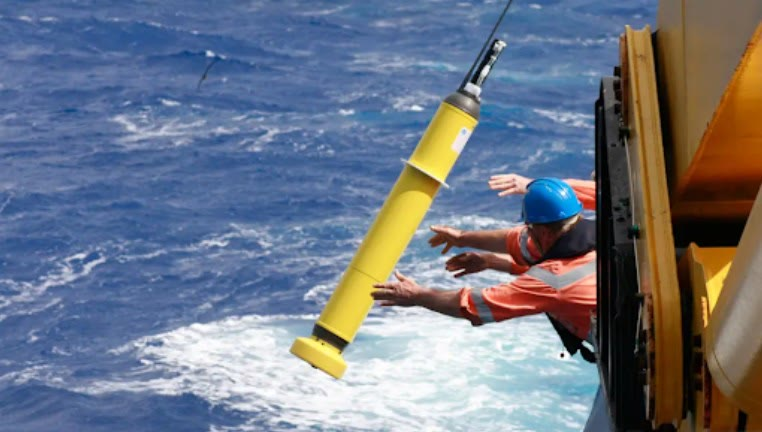
\includegraphics[width=\linewidth]{images/book5/b3-argo-deploy.jpg}

{\scriptsize Un flotteur Argo mis à l'eau depuis le bord d'un navire de recherche (NOAA
Global Ocean Monitoring and Observing Program, domaine public).}
\end{minipage}
\end{inthefield}
% ledger: argo:fleet, noaa:argo-25, photo:b3-argo-deploy

\section{Marées océaniques}\label{sec:b3:ocean-dynamics:tides}

Deux fois par jour, un peu moins d'une heure plus tard chaque jour, la mer monte
et descend. Les volumes de physique expliquent la force de marée~: l'attraction
de la Lune est plus forte sur le côté proche de la Terre qu'en son centre, et
plus faible sur le côté éloigné, de sorte que, par rapport au centre, l'eau est
tirée vers l'extérieur le long de la droite joignant la Lune, des deux côtés.

\begin{definition}[Marée d'équilibre~; composante de marée]\label{def:b3:ocean-dynamics:tides}
La \emph{marée d'équilibre}\index{marée d'équilibre} est la forme que prendrait la
surface d'un océan recouvrant toute la Terre s'il suivait instantanément le
potentiel générateur de marée, sans inertie. Une \emph{composante de
marée}\index{composante de marée} est l'un des termes harmoniques, chacun
de fréquence fixe imposée par les mouvements de la Lune et du Soleil, avec
une amplitude et une phase propres à chaque lieu, dont la somme forme la marée~; elles
se désignent par une lettre et le nombre de cycles par jour, comme M$_2$, la
composante lunaire principale semi-diurne.
\end{definition}

\begin{theorem}[Marée d'équilibre de la Lune]\label{thm:b3:ocean-dynamics:equilibrium-tide}
Pour la Lune, de masse $M$, située à la distance $d$ du centre de la Terre,
de masse $M_E$ et de rayon $a$, la \omterm{def:b3:ocean-dynamics:tides}{marée d'équilibre} à un angle $\theta$ du
point sous la Lune vaut
\[
\eta = K\,\frac{3\cos^2\theta - 1}{2},\qquad
K = \frac{M}{M_E}\Big(\frac{a}{d}\Big)^3 a .
\]
\end{theorem}

\begin{proof}
Le potentiel de la Lune en un point situé à la distance $a$ du centre de la
Terre et à l'angle $\theta$ vaut $-GM/s$, avec $s^2 = d^2 - 2ad\cos\theta +
a^2$. En développant en $a/d$, $1/s = (1/d)[1 + (a/d)\cos\theta + (a/d)^2
(3\cos^2\theta - 1)/2 + \cdots]$. Le premier terme est une constante~; le second
est un champ uniforme, celui qui accélère la Terre entière sur son orbite
autour du centre de masse commun, et n'a aucun effet par rapport à la Terre.
Ce qui reste est le potentiel générateur de marée $\Phi_T = -(GMa^2/d^3)(3
\cos^2\theta - 1)/2$. À l'équilibre, la surface de la mer est une surface de
potentiel total constant, $g\eta + \Phi_T = C$, avec $g = GM_E/a^2$, donc
$\eta = (M/M_E)(a^4/d^3)(3\cos^2\theta - 1)/2 + C/g$. La moyenne de
$3\cos^2\theta - 1$ sur la sphère est nulle~; le volume d'eau étant
fixé, $C = 0$.
\end{proof}

Avec le rapport des masses $0.0123$, $d = \qty{384400}{km}$ et $a =
\qty{6371}{km}$, $K = \qty{0.357}{m}$~: la mer s'élève de \qty{0.36}{m}
sous la Lune et du côté opposé, et s'abaisse de \qty{0.18}{m} sur le
grand cercle intermédiaire, soit un marnage de \qty{0.54}{m}. À la latitude $\varphi$, avec
la Lune à la déclinaison $\delta$ et à l'angle horaire $H$, $\cos\theta =
\sin\varphi\sin\delta + \cos\varphi\cos\delta\cos H$. Lorsque la Terre tourne
sous les deux renflements, un lieu connaît deux pleines mers par jour lunaire,
\qty{24}{h} \qty{50}{min}~: la marée semi-diurne. Lorsque la Lune se trouve
au nord ou au sud de l'équateur, les deux renflements sont inclinés, et les deux pleines mers
d'une même journée sont inégales, comme le montre la figure ci-dessous. Le Soleil soulève
une marée de même forme, \num{0.46} fois plus grande~; les deux s'ajoutent à la nouvelle
Lune et à la pleine Lune, en vives-eaux, et se compensent en partie aux quadratures.
% ledger: moon5:orbit, earth:Rmean, stewart:tide-equilibrium (computed in figdata/bachelor-3/tides.py)

\begin{omfigure}
\begin{tikzpicture}
\begin{groupplot}[group style={group size=2 by 1, horizontal sep=1.9cm},
  tick label style={font=\scriptsize}, label style={font=\small},
  legend style={font=\scriptsize, draw=none, fill=none}]
\nextgroupplot[width=0.40\linewidth, height=0.40\linewidth, axis equal image, hide axis,
  clip=false, xmin=-1.3, xmax=2.0, ymin=-1.25, ymax=1.25]
% computed in figdata/bachelor-3/tides.py
\addplot[fill=omThm!12, draw=omThm, thick] table[x=x, y=y] {figdata/out/bachelor-3-tides-bulge.dat};
\addplot[black, fill=black!10, domain=0:360, samples=91] ({cos(x)}, {sin(x)});
\draw[->, >=stealth, thick] (axis cs:1.25,0) -- (axis cs:1.95,0);
\node[above, font=\scriptsize, align=center] at (axis cs:1.6,0.08) {vers la\\Lune};
\node[font=\scriptsize] at (axis cs:0,0) {Terre};
\nextgroupplot[width=0.54\linewidth, height=0.40\linewidth, xlabel={temps (\unit{h})},
  ylabel={$\eta$ (\unit{m})}, xmin=0, xmax=49.6, xtick={0,12,24,36,48}, ymin=-0.2, ymax=0.4,
  legend style={at={(axis cs:12.4,0.39)}, anchor=north}, legend cell align=left, legend columns=2]
\addplot[omDef, thick] table[x=t, y=eta0] {figdata/out/bachelor-3-tides-series.dat};
\addlegendentry{$\delta = 0$}
\addplot[omThm, thick] table[x=t, y=eta20] {figdata/out/bachelor-3-tides-series.dat};
\addlegendentry{$\delta = \ang{20}$}
\addplot[black!50, thin, forget plot] coordinates {(0,0) (49.6,0)};
\end{groupplot}
\end{tikzpicture}

\par\smallskip{\small À gauche, la \omterm{def:b3:ocean-dynamics:tides}{marée d'équilibre} de la Lune, dans le plan
qui contient la Lune, le renflement étant exagéré environ deux millions de fois.
À droite, la \omterm{def:b3:ocean-dynamics:tides}{marée d'équilibre} à \ang{45}~N sur deux jours lunaires, avec la
Lune sur l'équateur (en bleu) et à la déclinaison \ang{20}~N (en rouge)~: le second
cas présente une pleine mer bien plus haute que l'autre, soit l'inégalité
diurne.}\label{fig:b3:ocean-dynamics:equilibrium-tide}
\end{omfigure}
% ledger: moon5:orbit, stewart:tide-constituents

L'analyse harmonique de la \omterm{def:b3:ocean-dynamics:tides}{marée d'équilibre} en donne les composantes. Les
cinq plus grandes, avec leurs amplitudes d'équilibre, sont données dans le tableau ci-dessous.
Au moins 39 composantes sont nécessaires pour prédire la marée d'un port à un millième de
son plus grand terme, et un marégraphe doit fonctionner plus de 18.6~ans, soit la période
de la modulation des marées lunaires, pour toutes les séparer.

\begin{center}
\small
\begin{tabular}{llrr}
\hline
composante & origine & période (\unit{h}) & amplitude d'équilibre (\unit{m}) \\
\hline
M$_2$ & principale lunaire, semi-diurne & \num{12.4206} & \num{0.2423} \\
S$_2$ & principale solaire, semi-diurne & \num{12.0000} & \num{0.1128} \\
N$_2$ & lunaire elliptique, semi-diurne & \num{12.6584} & \num{0.0464} \\
K$_1$ & luni-solaire, diurne & \num{23.9344} & \num{0.1416} \\
O$_1$ & principale lunaire, diurne & \num{25.8194} & \num{0.1005} \\
\hline
\end{tabular}
\end{center}
% ledger: stewart:tide-constituents, stewart:tide-prediction

La marée réelle n'est pas la \omterm{def:b3:ocean-dynamics:tides}{marée d'équilibre}. Pour maintenir un renflement sous la Lune
sur l'équateur, la marée devrait faire le tour de la Terre en un jour lunaire,
à environ \qty{460}{m/s}, vitesse qu'une longue onde de gravité n'atteint que
dans un océan de \qty{22}{km} de profondeur~; et les continents l'arrêtent. La marée est
plutôt une longue onde forcée, ballottant dans chaque bassin près de la résonance, et la
rotation de la Terre la fait tourner autour du bassin.
% ledger: stewart:tide-prediction

\begin{definition}[Onde de Kelvin]\label{def:b3:ocean-dynamics:kelvin-wave}
Une \emph{onde de Kelvin}\index{onde de Kelvin} océanique est une longue onde de gravité
qui se propage le long d'une côte, ou de l'équateur, sans vitesse
perpendiculaire à elle, sa hauteur décroissant exponentiellement en s'éloignant de la côte sur le
rayon de Rossby. Le long d'une côte, la côte reste à sa droite dans
l'hémisphère Nord, et à sa gauche dans l'hémisphère Sud.
\end{definition}

\begin{theorem}[Onde de Kelvin côtière]\label{thm:b3:ocean-dynamics:kelvin}
Dans un océan de profondeur uniforme $H$ sur un plan $f$, avec $f > 0$, délimité par
une côte rectiligne le long de $y = 0$ et occupant $y > 0$, les équations linéaires de l'eau peu profonde
admettent des solutions avec $v = 0$
\[
\eta = \mathrm e^{-y/L_R}F(x - ct),\qquad u = \frac{g}{c}\,\eta,\qquad
c = \sqrt{gH},\quad L_R = \frac{c}{f},
\]
pour tout profil $F$, et aucune solution avec $v = 0$ ne se propage dans la direction
$-x$.
\end{theorem}

\begin{proof}
Avec $v = 0$, les équations sont $\partial u/\partial t = -g\,\partial\eta/
\partial x$, $fu = -g\,\partial\eta/\partial y$ et $\partial\eta/\partial t
+ H\,\partial u/\partial x = 0$. La première et la troisième donnent $\partial^2
\eta/\partial t^2 = gH\,\partial^2\eta/\partial x^2$~: en $x$, chaque ligne
$y = $ const porte des ondes $F(x \mp ct)$ avec $c = \sqrt{gH}$, puis la
première équation donne $u = \pm(g/c)\eta$. La seconde devient $\partial\eta/
\partial y = \mp(f/c)\eta$, donc $\eta \propto \mathrm e^{\mp y/L_R}$. Avec
le signe supérieur, l'onde décroît en s'éloignant de la côte~; avec le signe inférieur, elle
croîtrait sans borne dans l'océan, ce qui est exclu. L'onde se propage vers
$+x$, l'océan à sa gauche et la côte à sa droite.
\end{proof}

En haute mer, à \qty{4000}{m} de profondeur, $c = \qty{198}{m/s}$ et le
rayon de Rossby vaut environ \qty{2000}{km} aux moyennes latitudes~: la marée
balaie tout un bassin. Sur une mer épicontinentale de \qty{50}{m} de profondeur, $c =
\qty{22}{m/s}$, le rayon de Rossby est inférieur à \qty{200}{km}, et une
longueur d'onde de M$_2$ vaut environ \qty{1000}{km}. Dans un golfe, la marée qui entre
le long d'une côte sous forme d'\omterm{def:b3:ocean-dynamics:kelvin-wave}{onde de Kelvin} revient le long de la côte opposée, toujours avec la
côte à sa droite~; les deux ondes s'annulent en des points intermédiaires.

\begin{definition}[Point amphidromique~; ligne cotidale~; ligne d'égale amplitude]\label{def:b3:ocean-dynamics:amphidrome}
Un \emph{point amphidromique}\index{point amphidromique} est un point où
l'amplitude d'une \omterm{def:b3:ocean-dynamics:tides}{composante de marée} est nulle et autour duquel sa pleine mer
tourne. Une \emph{ligne cotidale}\index{ligne cotidale} relie les lieux où la
pleine mer d'une composante survient au même instant~; une \emph{ligne
d'égale amplitude}\index{ligne d'égale amplitude} relie les lieux de même marnage. Les lignes cotidales
rayonnent à partir des points amphidromiques~; les lignes d'égale amplitude les entourent.
\end{definition}

\begin{omfigure}
\centering
\begin{tikzpicture}
\begin{axis}[width=0.96\linewidth, height=0.35\linewidth, axis equal image,
  xmin=0, xmax=1600, ymin=0, ymax=400, xtick={0,400,800,1200,1600}, ytick={0,200,400},
  xlabel={distance le long du chenal (\unit{km})}, ylabel={largeur (\unit{km})},
  tick label style={font=\scriptsize}, label style={font=\small}]
% computed in figdata/bachelor-3/tides.py
\addplot[omDef!70, densely dashed, unbounded coords=jump] table[x=x, y=y] {figdata/out/bachelor-3-tides-cor.dat};
\pgfplotsinvokeforeach{30,60,90,120,150,180,210,240,270,300,330}{
  \addplot[omThm, thin, unbounded coords=jump] table[x=x, y=y] {figdata/out/bachelor-3-tides-cot-#1.dat};
}
\addplot[omThm, very thick, unbounded coords=jump] table[x=x, y=y] {figdata/out/bachelor-3-tides-cot-0.dat};
\addplot[only marks, mark=*, mark size=2pt] table[x=x, y=y] {figdata/out/bachelor-3-tides-amph.dat};
\addplot[->, >=stealth, very thick, domain=20:310, samples=60] ({742.7+70*cos(x)}, {200+70*sin(x)});
\end{axis}
\end{tikzpicture}

\par\smallskip{\small Deux \omterm{def:b3:ocean-dynamics:kelvin-wave}{ondes de Kelvin} de la marée M$_2$ dans un chenal fictif
large de \qty{400}{km} et profond de \qty{50}{m} à \ang{55}~N, l'une allant vers l'est le long de la
côte sud, l'autre vers l'ouest le long de la côte nord.
En rouge, les \omterm{def:b3:ocean-dynamics:amphidrome}{lignes cotidales}, toutes les \ang{30} de phase (environ une heure), la
plus épaisse correspondant à la pleine mer à l'origine des temps~; en bleu pointillé, les
\omterm{def:b3:ocean-dynamics:amphidrome}{lignes d'égale amplitude}, tous les cinquièmes de l'amplitude d'une onde à sa côte.
Les \omterm{def:b3:ocean-dynamics:amphidrome}{points amphidromiques} (marques) se trouvent sur la ligne médiane, distants d'une demi-longueur d'onde,
soit \qty{495}{km} d'écart, et la pleine mer tourne autour
d'eux dans le sens antihoraire (flèche).}\label{fig:b3:ocean-dynamics:amphidromes}
\end{omfigure}

Les cartes de la marée océanique établies par altimétrie satellitaire, précises à
environ \qty{2}{cm} en haute mer, montrent partout cette structure~: la crête de M$_2$
tourne dans le sens antihoraire autour des amphidromes des bassins de l'hémisphère Nord
et dans le sens horaire dans l'hémisphère Sud, et les plus forts marnages sont sur les
côtes. Les marées dissipent \qty{3.75}{TW}, dont \qty{3.5}{TW} dans l'océan, environ
deux tiers de l'énergie de M$_2$ sur les plateaux et dans les mers peu profondes,
et un tiers par des ondes internes en haute mer. Cette énergie
allonge le jour d'environ \qty{2.07}{ms} par siècle et éloigne la Lune de
\qty{3.86}{cm} par an~; la part perdue en haute mer contribue au mélange,
en alimentant une partie du mélange qui, dans le \omterm{def:b3:ocean-dynamics:abyssal}{modèle de Stommel--Arons}, entretient
la circulation abyssale.
% ledger: stewart:tide-prediction


\section{Exercices}

\begin{exercise}[$\star$]\label{exo:b3:ocean-dynamics:1}
Une tension de vent d'ouest de \qty{0.12}{Pa} souffle sur la mer à \ang{40}~N
($\rho = \qty{1025}{kg/m^3}$, $\Omega = \qty{7.292115e-5}{rad/s}$).
Calculer le transport de volume d'Ekman par mètre de largeur et sa direction,
ainsi que le transport à travers une section longue de \qty{1000}{km}, en sverdrups.
\end{exercise}

\begin{exercise}[$\star$]\label{exo:b3:ocean-dynamics:2}
Avec $A_z = \qty{0.05}{m^2/s}$, calculer la \omterm{def:b3:ocean-dynamics:ekman-pumping}{profondeur d'Ekman} à \ang{45}~N. Quelle
fraction du courant de surface subsiste à cette profondeur~?
\end{exercise}

\begin{exercise}[$\star$]\label{exo:b3:ocean-dynamics:3}
À \ang{30}~N, le rotationnel de la tension du vent vaut \qty{-1e-7}{Pa/m} à travers un
bassin large de \qty{5000}{km} ($a = \qty{6371}{km}$). Calculer $\beta$, le
transport de Sverdrup par unité de largeur et le transport total, avec sa
direction.
\end{exercise}

\begin{exercise}[$\star$]\label{exo:b3:ocean-dynamics:4}
À partir des périodes de M$_2$ et de S$_2$, calculer la période du cycle des
marées de vives-eaux et de mortes-eaux, c'est-à-dire le temps entre deux alignements des deux
composantes.
\end{exercise}

\begin{exercise}[$\star\star$]\label{exo:b3:ocean-dynamics:5}
Une tension de vent d'ouest croît linéairement de 0 à \ang{35}~N jusqu'à
\qty{0.1}{Pa} à \ang{45}~N, \qty{1110}{km} plus au nord. Calculer le \omterm{def:b3:ocean-dynamics:ekman-pumping}{pompage d'Ekman} à
\ang{40}~N, en conservant les deux termes de la \cref{prop:b3:ocean-dynamics:pumping}, en
mètres par an. L'eau est-elle poussée vers le haut ou vers le bas~?
\end{exercise}

\begin{exercise}[$\star\star$]\label{exo:b3:ocean-dynamics:6}
Dans un gyre de Stommel avec $r = \qty{2e-6}{s^{-1}}$ et $\beta =
\qty{2e-11}{m^{-1}.s^{-1}}$, calculer la largeur $\delta_S$. Si le courant de bord
transporte \qty{30}{\sverdrup} dans les \qty{800}{m} supérieurs, sur une
largeur $\delta_S$, quelle est sa vitesse moyenne~?
\end{exercise}

\begin{exercise}[$\star\star$]\label{exo:b3:ocean-dynamics:7}
Calculer la largeur de Munk $\delta_M$ et la largeur du jet dirigé vers le nord,
$(2\pi/\sqrt3)\,\delta_M$, à \ang{30}~N pour $A_H = \qty{e4}{m^2/s}$. Comment
varie la largeur si $A_H$ est huit fois plus petit~?
\end{exercise}

\begin{exercise}[$\star\star$]\label{exo:b3:ocean-dynamics:8}
Deux stations distantes de \qty{80}{km} sont situées sur une ligne allant de l'ouest ($A$) à
l'est ($B$) à \ang{36}~N. Par rapport à la surface \qty{1000}{dbar}, l'anomalie
géopotentielle de la surface de la mer vaut \qty{14.5}{J/kg} en $A$ et
\qty{21.3}{J/kg} en $B$. Calculer le courant de surface par rapport à
\qty{1000}{dbar} et sa direction. Quelle station possède la colonne d'eau
la plus chaude~?
\end{exercise}

\begin{exercise}[$\star\star$]\label{exo:b3:ocean-dynamics:9}
Avec la \omterm{def:b3:ocean-dynamics:tides}{marée d'équilibre} de la Lune, $K = \qty{0.357}{m}$, et le rapport
\num{0.46} de la marée solaire à la marée lunaire, calculer le marnage d'équilibre
(pleine mer sous les astres moins basse mer à \ang{90}) en vives-eaux et
en mortes-eaux, ainsi que leur rapport.
\end{exercise}

\begin{exercise}[$\star\star\star$]\label{exo:b3:ocean-dynamics:10}
Sur le plan $\beta$ équatorial, $f = \beta_0y$ avec $\beta_0 =
2\Omega/a$. Montrer que l'\omterm{def:b3:ocean-dynamics:kelvin-wave}{onde de Kelvin} $\eta = G(y)F(x - ct)$, $v = 0$,
devient $G = \exp(-\beta_0y^2/2c)$, piégée des deux côtés de l'équateur,
et se propage vers l'est. Calculer son échelle de piégeage $\sqrt{c/\beta_0}$ pour une
onde de vitesse \qty{2.5}{m/s}.
\end{exercise}

\begin{exercise}[$\star\star\star$]\label{exo:b3:ocean-dynamics:11}
(a)~Établir $V = a\tan\varphi\,W_0$ pour l'intérieur abyssal à partir de $\beta v =
f\,\partial w/\partial z$. (b)~Avec $W_0 = \qty{e-7}{m/s}$, calculer $V$ à
\ang{30}~N, ainsi que le transport total vers le pôle à travers un bassin
de \qty{5000}{km} de large. (c)~D'où doit provenir l'eau~?
\end{exercise}

\begin{exercise}[$\star\star\star$]\label{exo:b3:ocean-dynamics:12}
Un courant géostrophique $W_g = u_g + \mathrm iv_g$ s'écoule sur un fond marin plat en
$z = 0$, avec une viscosité turbulente $A_z$ et une condition de non-glissement au fond.
(a)~Montrer que $W = W_g(1 - \mathrm e^{-(1+\mathrm i)z/\delta})$, $\delta =
\sqrt{2A_z/f}$. (b)~Montrer que le défaut de transport de cette couche d'Ekman de fond
pompe la vitesse verticale $w = \tfrac12\delta\zeta_g$ dans l'intérieur,
$\zeta_g$ la vorticité du courant géostrophique. (c)~Pour
$A_z = \qty{0.01}{m^2/s}$, $f = \qty{e-4}{s^{-1}}$ et un océan
d'une profondeur de \qty{4000}{m}, calculer $\delta$, le taux de ralentissement $r =
f\delta/2H$, et son inverse en jours.
\end{exercise}
% ledger: earth:Rmean, geod5:grs80-defining, stewart:tide-constituents, stewart:tide-equilibrium

\section{Problème~: un gyre dans la mer d'Ammar}

\begin{problem}[{Problème du week-end --- pompage d'Ekman, transport de Sverdrup,
le courant de bord ouest et la marée d'un océan fictif}]
\label{pb:b3:ocean-dynamics:1}
La mer d'Ammar est un bassin océanique fictif, un rectangle allant de \ang{20} à
\ang{50}~N et \qty{6000}{km} de large, \qty{4000}{m} de profondeur. La tension du vent est
zonale, $\tau_x = -\tau_0\cos(\pi(\varphi - \ang{20})/\ang{30})$ avec $\tau_0
= \qty{0.1}{Pa}$. On prend $\rho = \qty{1025}{kg/m^3}$, $\Omega =
\qty{7.292115e-5}{rad/s}$, $a = \qty{6371}{km}$, $g = \qty{9.81}{m/s^2}$,
et, lorsqu'un plan $\beta$ est demandé, sa valeur à \ang{35}~N.

\medskip\noindent\textbf{Partie I --- La couche d'Ekman.}
\begin{enumerate}
\item Calculer la tension du vent à \ang{20}, \ang{35} et \ang{50}~N.
\item Calculer $f$ aux mêmes latitudes.
\item Calculer le transport volumique d'Ekman par unité de largeur à \ang{20} et
  \ang{50}~N, avec sa direction. Les transports convergent-ils ou divergent-ils dans
  le bassin~?
\item Avec $A_z = \qty{0.05}{m^2/s}$, calculer la \omterm{def:b3:ocean-dynamics:ekman-pumping}{profondeur d'Ekman} à \ang{35}~N.
\item Calculer le \omterm{def:b3:ocean-dynamics:ekman-pumping}{pompage d'Ekman} à \ang{35}~N, en mètres par seconde et par
  an.
\item Combien d'années ce pompage mettrait-il à faire descendre l'eau de surface
  de \qty{500}{m}~?
\end{enumerate}

\medskip\noindent\textbf{Partie II --- L'intérieur de Sverdrup.}
\begin{enumerate}[resume]
\item Calculer la longueur $L$ du bassin du sud au nord et $\beta$ à
  \ang{35}~N.
\item Calculer le rotationnel de la tension du vent à \ang{35}~N.
\item Calculer le transport de Sverdrup par unité de largeur à \ang{35}~N, avec sa
  direction.
\item Calculer le transport total de l'intérieur à travers le bassin à \ang{35}~N,
  en sverdrups.
\item Si cet écoulement est réparti sur les \qty{1000}{m} supérieurs, quelle est sa
  vitesse moyenne, et combien d'années une parcelle met-elle pour parcourir \qty{1000}{km}
  vers le sud~?
\item Montrer que $fw_E/\beta$ à \ang{35}~N donne le même transport, et expliquer
  pourquoi, avec la \omterm{def:b3:atmospheric-dynamics:pv}{vorticité potentielle} d'une colonne.
\end{enumerate}

\medskip\noindent\textbf{Partie III --- Le courant de bord ouest.}
\begin{enumerate}[resume]
\item Expliquer pourquoi le courant de retour ne peut pas longer le côté est du
  bassin.
\item Avec un frottement de fond $r = \qty{e-6}{s^{-1}}$, calculer la largeur
  de Stommel $\delta_S$.
\item Calculer le transport vers le nord par unité de largeur au mur ouest,
  $A(X/\delta_S - 1)$, et la vitesse moyenne s'il remplit les
  \qty{1000}{m} supérieurs.
\item À quelle distance du mur l'écoulement vers le nord s'arrête-t-il~?
\item Calculer le transport vers le nord de la couche limite de Stommel, et expliquer
  pourquoi il reste inférieur au transport de l'intérieur d'environ
  \qty{1.5}{\sverdrup}.
\item Avec $A_H = \qty{5e3}{m^2/s}$, calculer $\delta_M$ et la largeur du jet
  de Munk dirigé vers le nord.
\item Le jet de Munk transporte $1 + \mathrm e^{-\pi/\sqrt3}$ fois le transport de
  l'intérieur. Calculer ce transport, puis préciser où va l'excédent.
\end{enumerate}

\medskip\noindent\textbf{Partie IV --- La marée de la mer d'Ammar.}
\begin{enumerate}[resume]
\item Calculer la vitesse d'une \omterm{def:b3:ocean-dynamics:kelvin-wave}{onde de Kelvin} dans le bassin et le rayon de
  Rossby à \ang{35}~N.
\item Calculer la longueur d'onde de l'\omterm{def:b3:ocean-dynamics:kelvin-wave}{onde de Kelvin} M$_2$.
\item Combien de temps une \omterm{def:b3:ocean-dynamics:kelvin-wave}{onde de Kelvin} met-elle pour faire le tour des côtes du
  bassin, et combien de périodes de M$_2$ cela représente-t-il~?
\item À quelle vitesse la \omterm{def:b3:ocean-dynamics:tides}{marée d'équilibre} devrait-elle parcourir le cercle
  de \ang{35}~N pour rester sous la Lune, et à quelle profondeur d'océan
  une onde longue se propage-t-elle à cette vitesse~?
\item Où s'attend-on à trouver le \omterm{def:b3:ocean-dynamics:amphidrome}{point amphidromique} du bassin, et dans quel
  sens la pleine mer tourne-t-elle autour de lui~?
\item Calculer l'amplitude d'équilibre semi-diurne à \ang{35}~N, $\tfrac34
  K\cos^2\varphi$, avec $K = \qty{0.357}{m}$, pour la Lune sur l'équateur.
\item Donner le transport du courant de bord ouest qui ferme le gyre de la
  mer d'Ammar.
\end{enumerate}
\end{problem}
% ledger: earth:Rmean, geod5:grs80-defining, stewart:tide-constituents
